\documentclass{beamer}
\usetheme{metropolis} 
\usepackage{caption}
\usepackage[utf8]{inputenc}


\title{\huge Konobi}
\date{}
\subtitle{Software Development Methods project}
\author{Lorenzo Basile, Irene Brugnara, Roberto Corti, Arianna Tasciotti}

\begin{document}
	
  \maketitle
  \section{Introduction}
  
  \begin{frame}{Our project}
    The goal of our project was to develop a command line version of \textbf{Konobi}, a board game for two players. The project also contains a client-server version of the game, which allows the two players to play remotely.
    \vspace{0.7cm}
    \pause
    \\What tools did we use?
    \begin{itemize}
	    \item Java 15
	    \item Gradle
	    \item TravisCI
	    \item Git \& GitHub
    \end{itemize}

  \end{frame}
  
  \begin{frame}{Konobi}
	    Konobi is a drawless game and it can be played either on a go board or a chess board.
	    \\Two players, black and white, take turns at placing stones of their color on the board, starting with black. The aim of the players is to build chains of connected stones of their color.
	    \vspace{0.5cm}
	    \pause
	    \\The game is won by the first player who connects the two opposite edges of the board.
	    \begin{itemize}
	    \item Black: top $\leftrightarrow$ bottom
	    \item White: left $\leftrightarrow$ right
	    \end{itemize}
   \end{frame}
      
   \begin{frame}{Connections}
     Two like-colored stones can be:
     \vspace{0.5cm}
    \begin{columns}
			\column{0.5\textwidth}
			\begin{figure}
				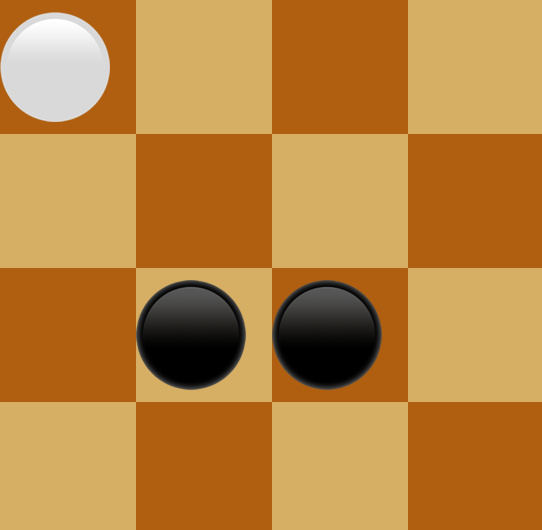
\includegraphics[scale=0.35]{images/strong.png}
				\caption*{Strongly connected}
			\end{figure}
					
			\column{0.5\textwidth}
			\begin{figure}
				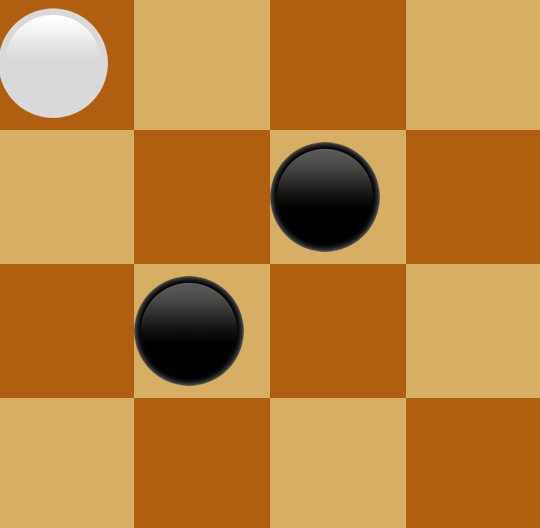
\includegraphics[scale=0.35]{images/weak.png}
				\caption*{Weakly connected}
			\end{figure}
		
	\end{columns}
	\vspace{0.7cm}
	A chain is a set of connected stones

      \end{frame}
      
      \begin{frame}{Placement rules}
     Not all moves are allowed:
     \begin{itemize}
     \item \textbf{Weak connections} to a certain stone are illegal unless it is impossible to make a placement that is both strongly connected to that stone and not weakly connected to another
     \item \textbf{Crosscut} placements are always illegal
     \end{itemize}
    \begin{columns}
			\column{0.5\textwidth}
			\begin{figure}
				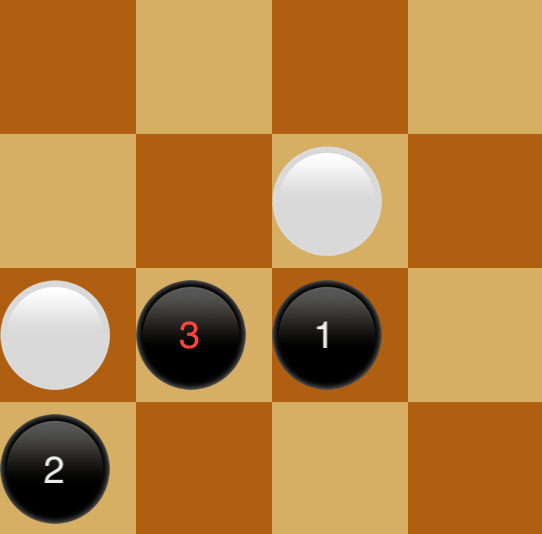
\includegraphics[scale=0.35]{images/legal_weak.png}
				\caption*{Legal weak connection}
			\end{figure}
					
			\column{0.5\textwidth}
			\begin{figure}
				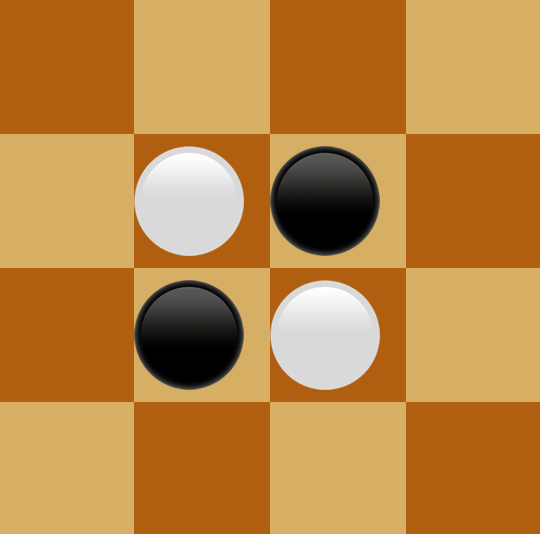
\includegraphics[scale=0.35]{images/crosscut.png}
				\caption*{Crosscut placement}
			\end{figure}
		
	\end{columns}
      \end{frame}
      
      \begin{frame}{Additional rules}
     \begin{itemize}
     \item \textbf{Pie rule}: at his first move, white can decide to switch colors with black instead of making a move.
     \item \textbf{Mandatory pass}: if a player cannot make a move (because of placement restrictions), he has to pass. It is guaranteed that at least one player can make a move.
     \end{itemize}
      \end{frame}
      
\section{Let's see a live demo}
      
      
      
      
      
      
\section{Basic entities}
\begin{frame}{The basic building block: \texttt{Cell}}

\begin{columns}
\column{0.6\textwidth}
\begin{itemize}
\item When a cell is constructed it is empty: no color is associated to it and \texttt{isOccupied} is \texttt{False}
\item When a stone is placed in the cell, a color is set and \texttt{isOccupied} becomes \texttt{True}
\end{itemize}
\vspace{0.8cm}
Development history:
\begin{itemize}
	\item From value \texttt{NONE} in enum \texttt{Color} to field \texttt{isOccupied} in class \texttt{Cell}
	\item Removed \texttt{Stone} data class
\end{itemize}

\column{0.4\textwidth}
\begin{figure}
	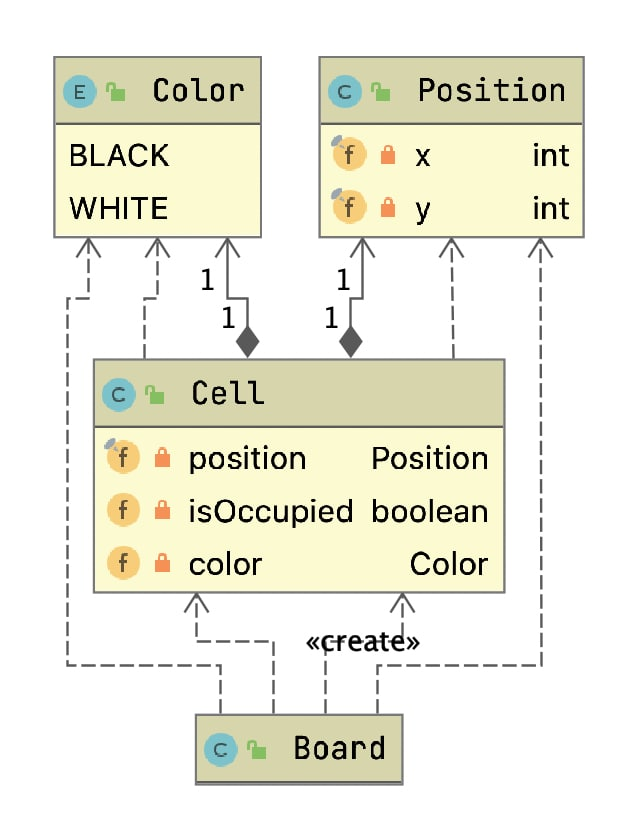
\includegraphics[scale=0.4]{images/cell-class.png}
\end{figure}

\end{columns}


\end{frame}




\begin{frame}{\texttt{Board}}

A \texttt{Board} is represented by a set of cells and extends \texttt{HashSet<Cell>} 

\vspace{0.5cm}
Reasons for this choice of data structure:
\begin{itemize}
    \item Usage of streams
    \item \texttt{Position} as attribute of \texttt{Cell}    
\end{itemize}


\end{frame}


\section{Connections}


\begin{frame}{Strong connections}


	in class \texttt{Position}:

	\begin{figure}
		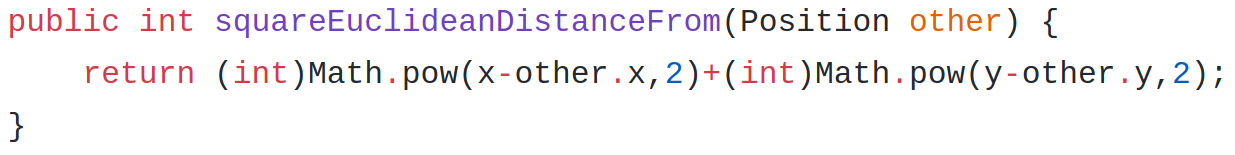
\includegraphics[scale=0.15]{images/position.png}
	\end{figure}



	in class \texttt{Cell}:

	\begin{figure}
		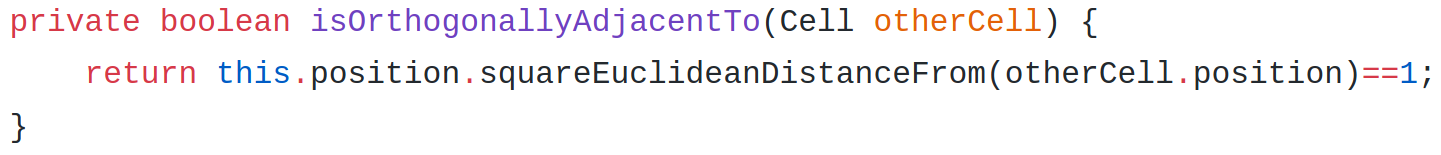
\includegraphics[scale=0.15]{images/cell1.png}
		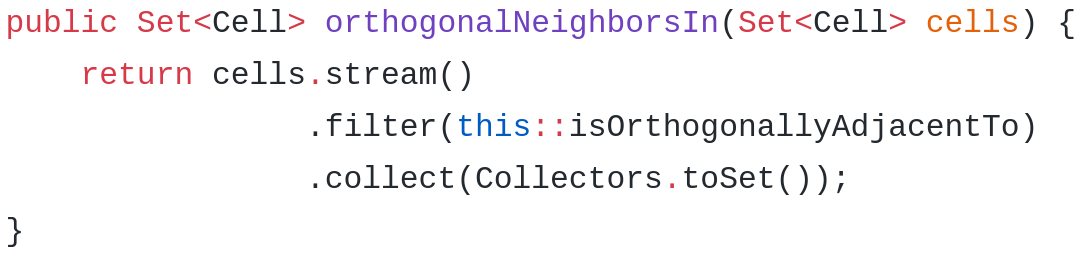
\includegraphics[scale=0.15]{images/cell2.png}
	\end{figure}

	
	in class \texttt{Board}:

	\begin{figure}
		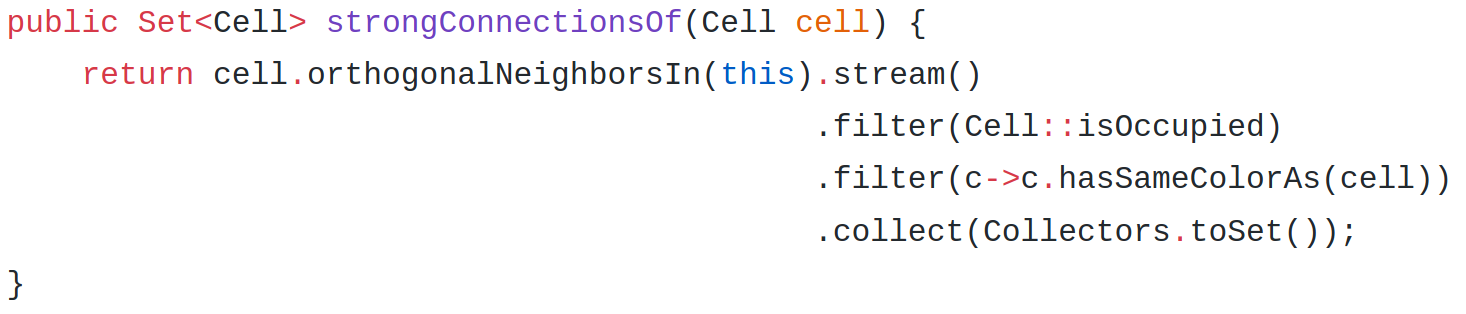
\includegraphics[scale=0.15]{images/board1.png}
	\end{figure}


	
\end{frame}

\begin{frame}{Weak connections}

	in class \texttt{Board}:
\begin{figure}
	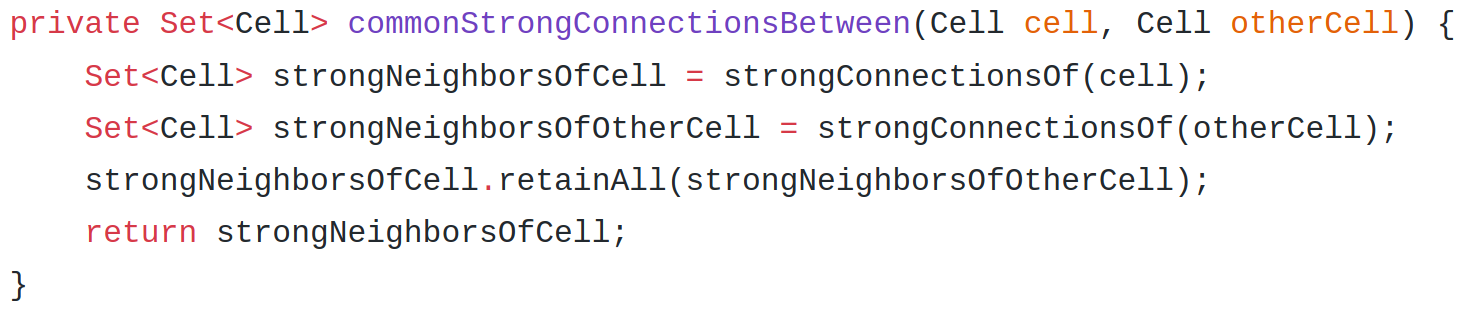
\includegraphics[width=0.74\textwidth]{images/board2.png}
	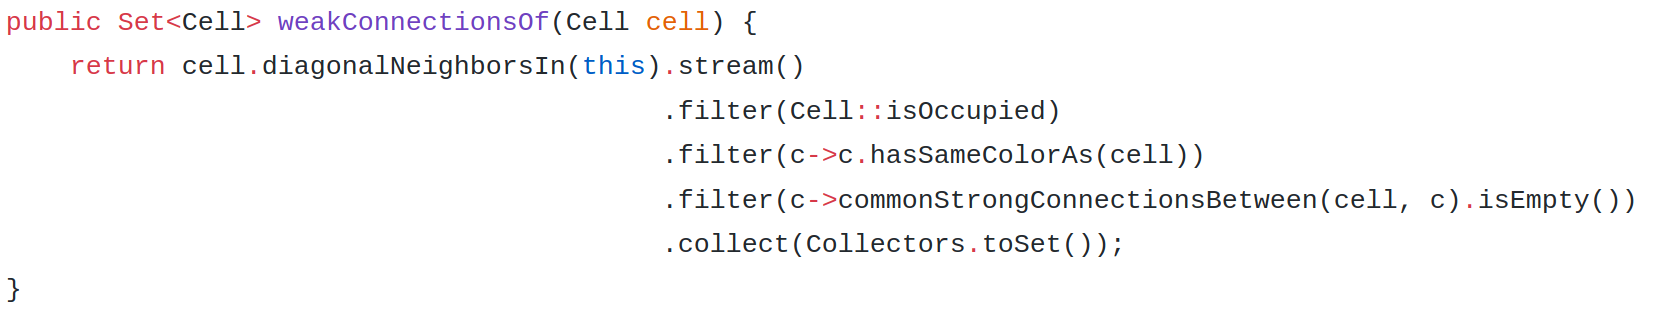
\includegraphics[width=1\textwidth]{images/board3.png}
\end{figure}

\end{frame}



\begin{frame}{Tests}
	Different test cases for diagonal adjacency (same for orthogonal):
\begin{columns}
\column{0.33\textwidth}
	\begin{figure}
		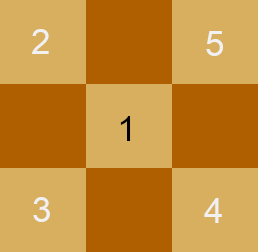
\includegraphics[scale=0.15]{images/inner.png}
		\\inner cell
	\end{figure}
\column{0.33\textwidth}
	\begin{figure}
		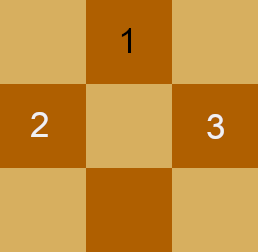
\includegraphics[scale=0.15]{images/edge.png}
		\\cell on edge
	\end{figure}
\column{0.33\textwidth}
	\begin{figure}
	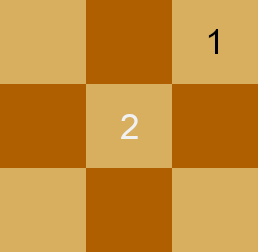
\includegraphics[scale=0.15]{images/corner.png}
    \\cell on corner
\end{figure}
\end{columns}
	\vspace{0.9cm}
	Example of tests for strong and weak connection: 
	\begin{columns}
		\column{0.5\textwidth}
		\begin{figure}
			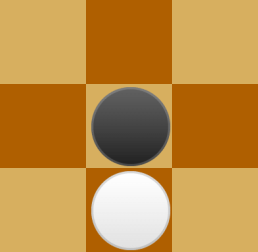
\includegraphics[scale=0.15]{images/test-strong-connection.png}
			
			the two stones are \\\textit{not} strongly connected
		\end{figure}
		
		\column{0.5\textwidth}
		\begin{figure}
			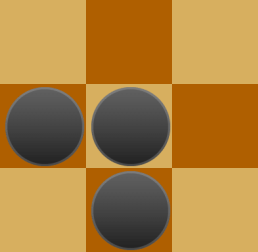
\includegraphics[scale=0.15]{images/test-weak-connection.png}
			
			the two stones are \\\textit{not} weakly connected
		\end{figure}
	\end{columns}
\end{frame}      
      
      
      
      
      
      
      
      
\section{Rules}

\begin{frame}{Placement rules: how to implement them?}
 A feature that Konobi has to provide is that a player must make a move which respects placement rules:
 \vspace{0.3cm}
 
 \begin{itemize}
  \item It's illegal to make a weak connection to a certain stone unless it's impossible to make a placement which is both strongly connected to that stone and not weakly connected to another (\textbf{Weak Connection Rule})
  \item It's illegal to make a 2x2 pattern of stones consisting of two diagonally adjacent Black stones and two diagonally adjacent White stones. (\textbf{Crosscut Rule})
 \end{itemize}

 \vspace{0.2cm}
 
 Initially, a \texttt{Rules} class was implemented... 
\end{frame}

\begin{frame}{Rules package}
 ...but later we realized that there could be a way to abstract
 \begin{figure}
  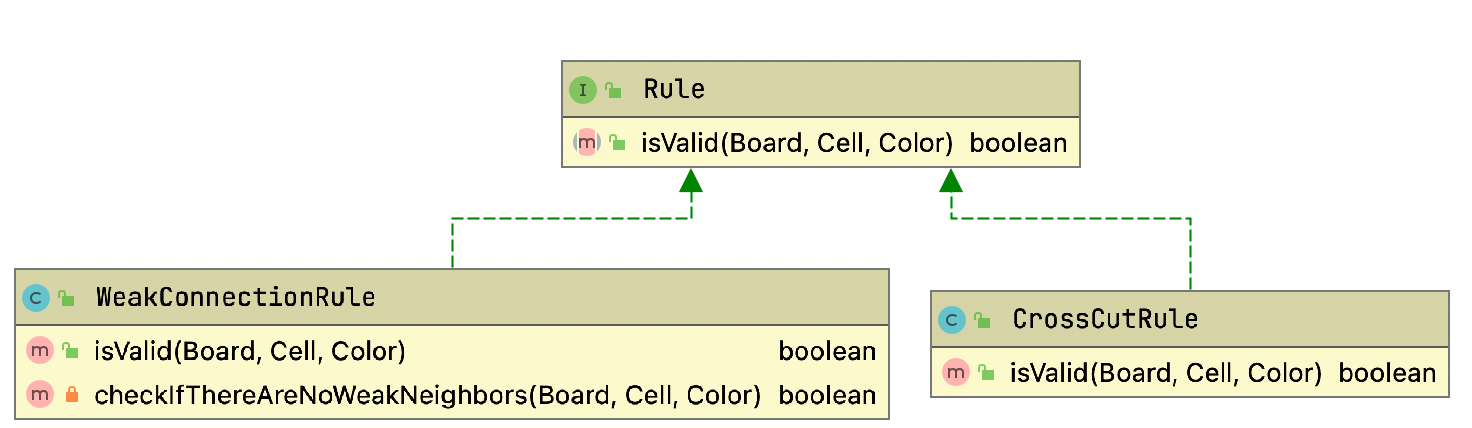
\includegraphics[scale=0.4]{images/rules-uml.png}
 \end{figure}
 
 For a given \texttt{Board}, the \texttt{isValid} method will check if it is legal to place a stone of a given \texttt{Color} in the \texttt{Cell}. \\
 \vspace{0.1cm}
 A \texttt{Rule} interface will allow the possibility to add new rules on the game.
 
\end{frame}

\begin{frame}[t]{How the rules were implemented }
 \begin{itemize}
  \item \texttt{WeakConnectionRule}
  \vspace{0.4cm}
  \
  \begin{figure}
   \center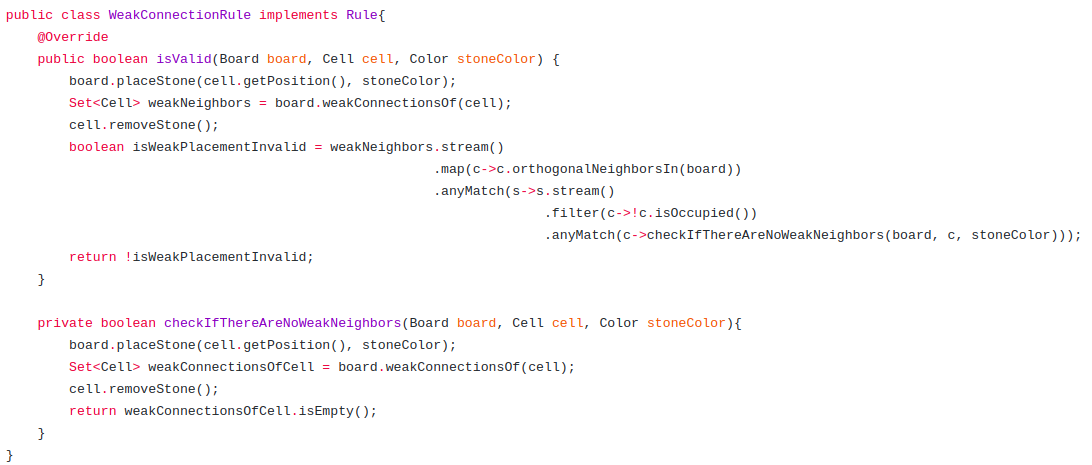
\includegraphics[scale=0.19]{images/weak-connection-rule-code.png}
  \end{figure}
  \item \texttt{CrossCutRule}
  \vspace{0.4cm}
  \begin{figure}
   \center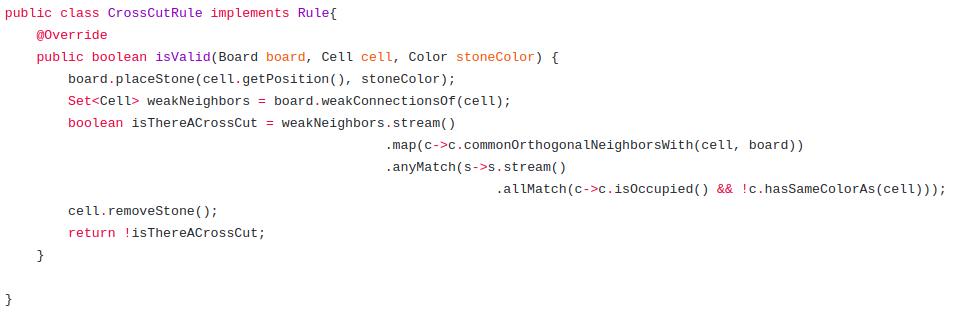
\includegraphics[scale=0.2]{images/cross-cut-rule-code.png}
  \end{figure}
 \end{itemize}
\end{frame}

\begin{frame}[t]{How the rules were tested }
 
 We implemented \texttt{WeakConnectionRule} and \texttt{CrossCutRule} by following TDD principles based on some examples...\\
 \vspace{0.1cm}
 \textbf{Legal moves}
 \begin{columns}
  \column{0.5\textwidth}
  %codice
  \begin{figure}[t]
   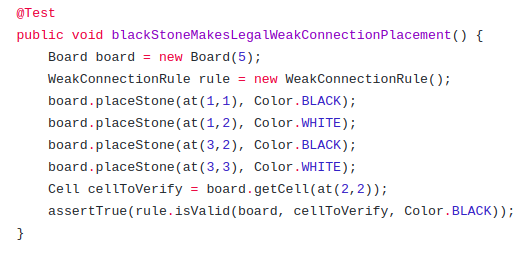
\includegraphics[scale=0.27]{images/test-legal-weak.png}
  \end{figure}
  \column{0.3\textwidth}
  %esempio
  \begin{figure}[t]
   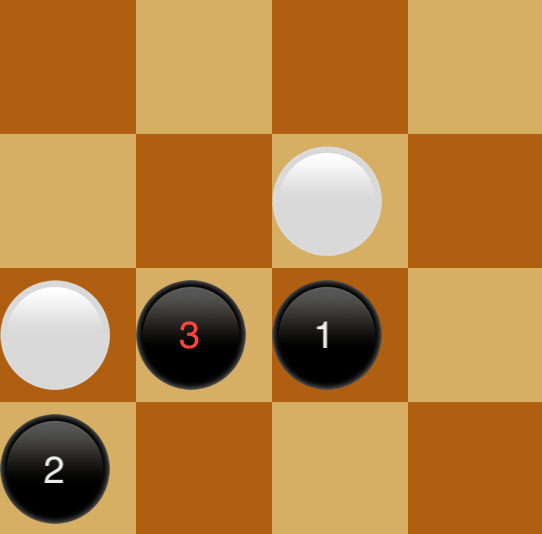
\includegraphics[scale=0.24]{images/legal_weak.png}
  \end{figure}
  
 \end{columns}
 
 \textbf{Illegal moves}
 \begin{columns}
  \column{0.3\textwidth}
  %codice
  \begin{figure}[t]
   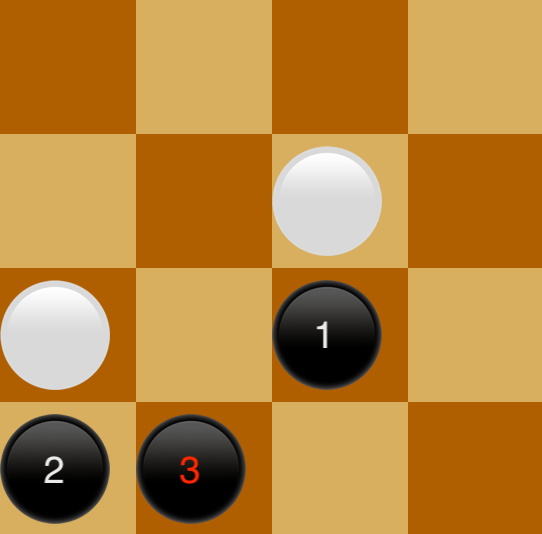
\includegraphics[scale=0.24]{images/illegal_weak.png}
  \end{figure}
  \column{0.5\textwidth}
  %esempio
  \begin{figure}
   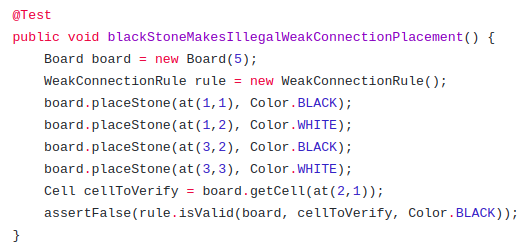
\includegraphics[scale=0.27]{images/test-illegal-weak.png}
  \end{figure}
  
 \end{columns}
 
 
 
 
\end{frame}

\begin{frame}{A new entity comes: \texttt{Referee}}
 \begin{columns}
  \column{0.5\textwidth}
  Given the logic of a valid move in \texttt{Rules} package, our aim was to group together all the methods needed to check if:
  \vspace{0.4cm}
  \begin{itemize}
   \item a given move is legal w.r.t. \texttt{WeakConnectionRule} and \texttt{CrossCutRule}
   \vspace{0.25cm}
   \item a winning chain is present
   \vspace{0.25cm}
   \item the current player has to pass
  \end{itemize}
  
  \column{0.5\textwidth}
  
  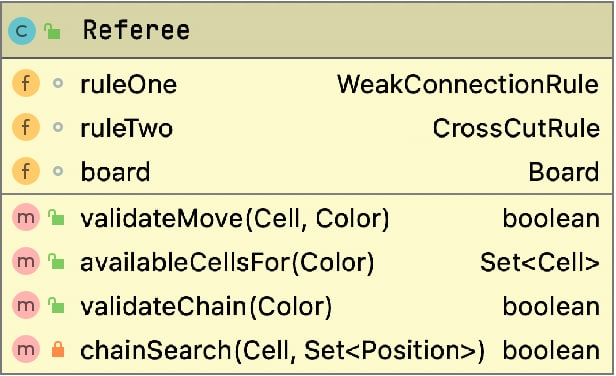
\includegraphics[scale=0.27]{images/referee-class.jpg}
  
 \end{columns}
\end{frame}

\begin{frame}{How to find a winning chain}
 \texttt{isThereaWinningChainFor} method is used to find a chain of a given \texttt{Color}.
 
 
 \begin{figure}
  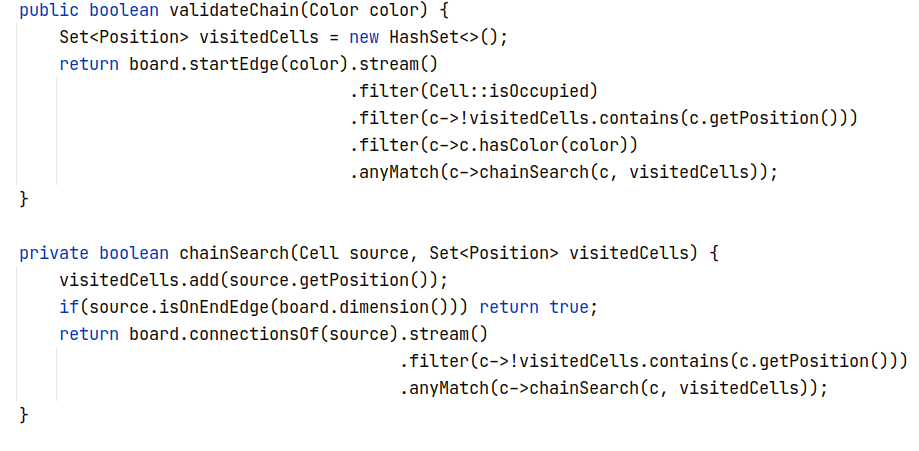
\includegraphics[scale=0.2, width=7cm]{images/chainsearch-code.png}
 \end{figure}
 
 \textbf{Recursive approach}: starting from all stones placed on the start edge, we explore the set of their connected stones inside the board until we arrive in the end edge.
\end{frame}



\section{InputOutput}

\begin{frame}{Handling user interaction: \texttt{InputTerminal} and \texttt{Display}}
 Classes \texttt{InputTerminal} and \texttt{Display} take care of game I/O.

 \begin{itemize}
  \item \texttt{Display}: communication with players through messages
   \item \texttt{InputTerminal}: management of player inputs
 \end{itemize}
 
   \begin{center}
       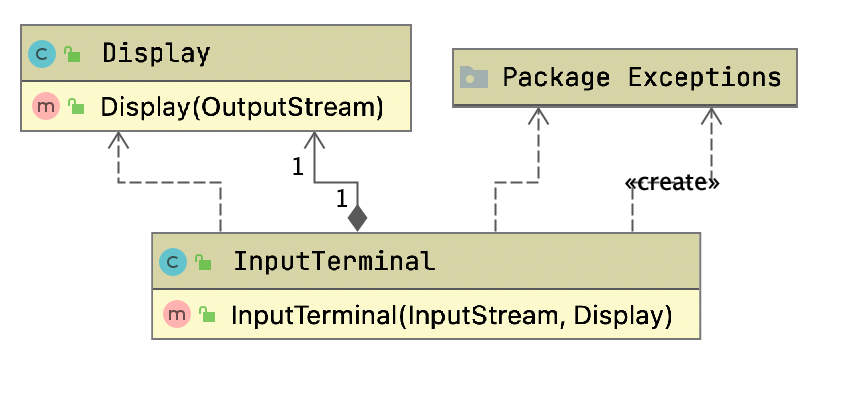
\includegraphics[scale=0.45]{images/inputoutput.png}
      \end{center}
\end{frame}

\begin{frame}{Sorting out exceptional events}

 Potential issues with user input:
 \begin{itemize}
  \item negative number (board dimension, move coordinates)
  \item wrong answer (pie rule requires "y" or "n")
  \item number format (string instead of an integer)
 \end{itemize}
 
 \vspace{0.7cm}
 
 How to deal with them:
 \begin{itemize}
  \item \texttt{throw} (and \texttt{catch}) custom exceptions extending \texttt{Exception} java class
 \end{itemize}
 
\end{frame}


\section{Game dynamics}


\begin{frame}{Building blocks for game dynamics}
   \begin{center}
       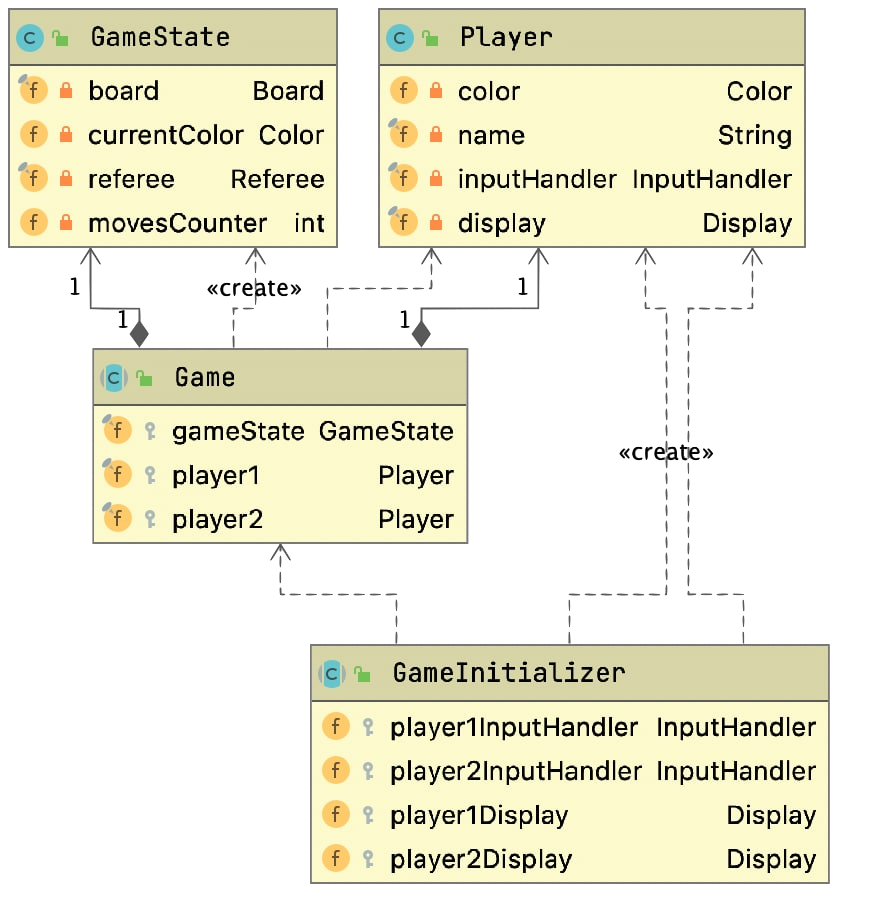
\includegraphics[scale=0.25]{images/game_uml.png}
      \end{center}

\end{frame}

\begin{frame}{Game flow management: \texttt{GameState}}
     
     \texttt{GameState} class keeps track of current state of the game.
     \vspace{0.5cm}
     \begin{center}
      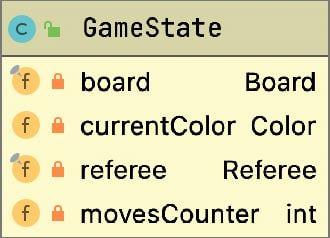
\includegraphics[scale=0.42]{images/gamestate.png}
     \end{center}
    
     \vspace{0.4cm}
   \texttt{GameState} acts as an intermediary between \texttt{Referee} and \texttt{Board} on one side and the higher-level class \texttt{Game} on the other  side.
     
\end{frame}

\begin{frame}{Game execution: core methods}  
 Based on the directives of \texttt{GameState}, \texttt{Game} manages the interactions with players.
 \\
      \pause
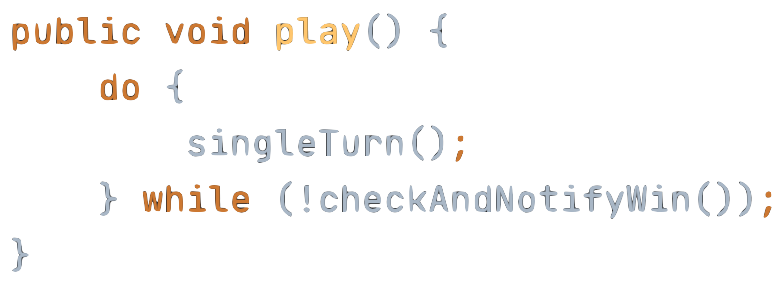
\includegraphics[scale=0.30]{images/play.png}
    \pause
 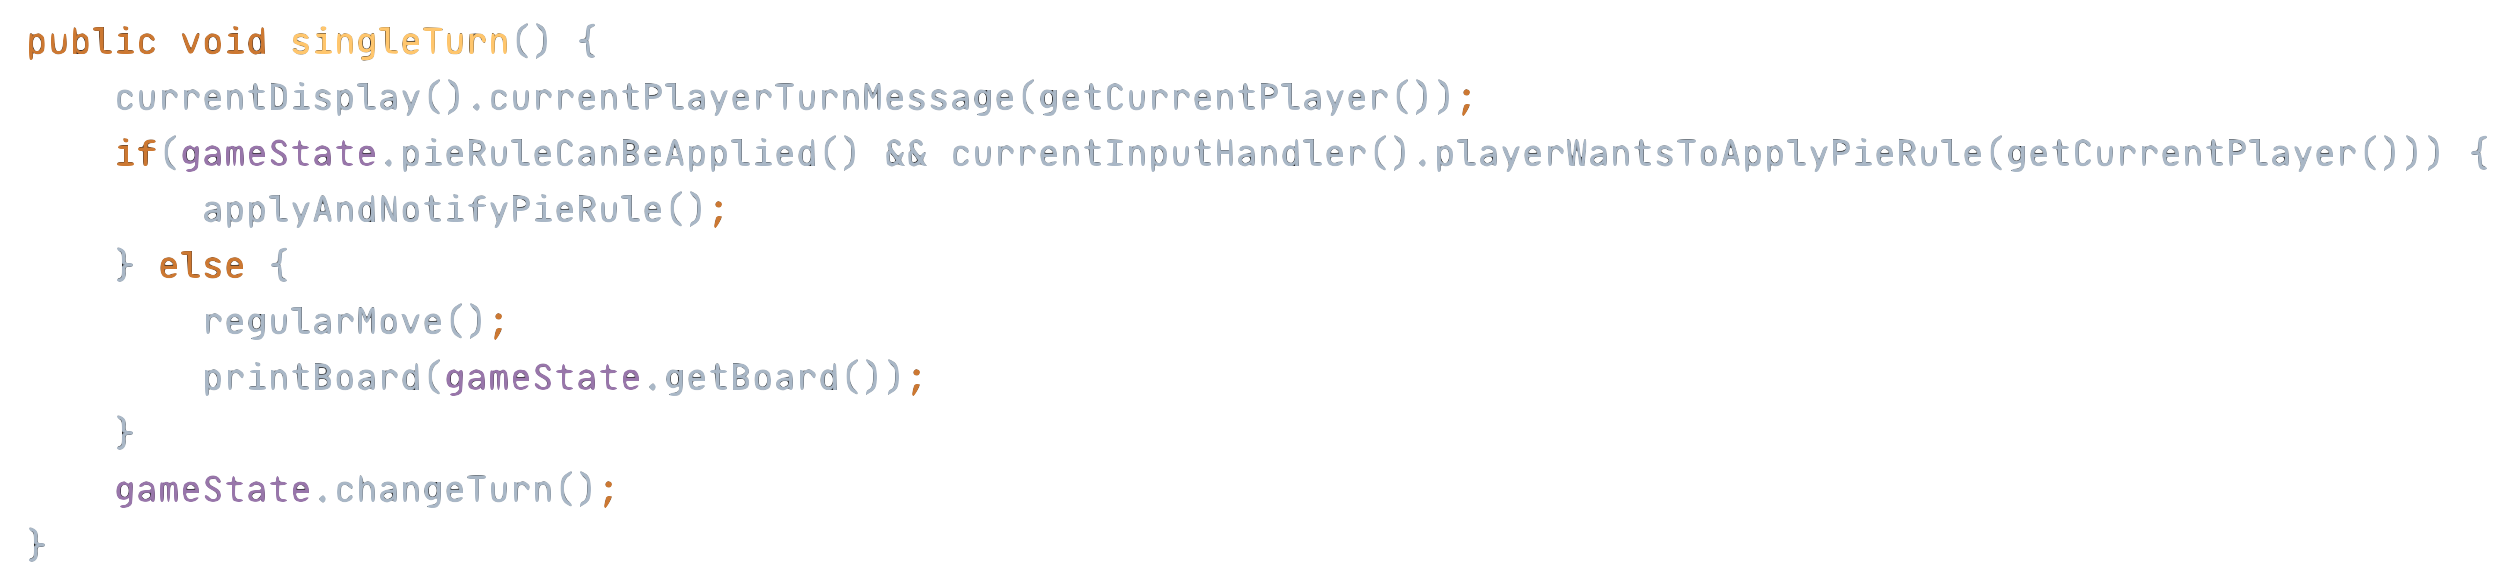
\includegraphics[scale=0.30]{images/singleturn.png}
 \pause
 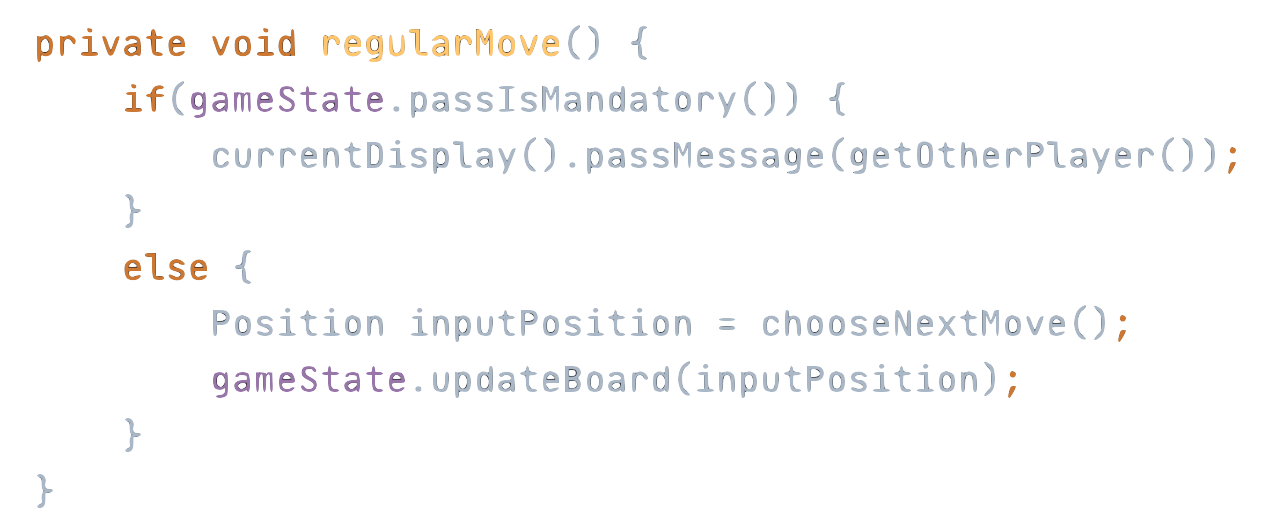
\includegraphics[scale=0.30]{images/regularmove.png}
\end{frame}

\begin{frame}{Preparing the game: \texttt{GameInitializer}}

 \begin{columns}
  \column{0.6\textwidth}
    Abstraction for  \texttt{Game} initialization:
   \begin{itemize}
    \item welcome message
    \item receiving input board dimension
    \item construct players
    \item construct game
    \item display player colors
   \end{itemize}
  \column{0.5\textwidth}
        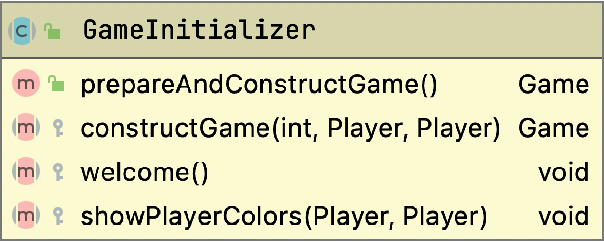
\includegraphics[scale=0.5]{images/gameinitializer.png}
     \end{columns}
\end{frame}

\section{Running the game}

\begin{frame}{Two versions of Konobi}
Konobi can be played by the two players on the same terminal or in a Client-Server version, with the two players connecting through \texttt{telnet} to a Server running the game.
\\ Code duplication between the two versions is avoided by exploiting polymorphism: abstract classes \texttt{Game} and \texttt{GameInitializer} allow for very general code in the form:
\\
\center 
\includegraphics[scale=0.5]{images/gameplay.png}
\end{frame}

\begin{frame}{Behind the scenes of \texttt{prepareAndConstructGame}}
\center 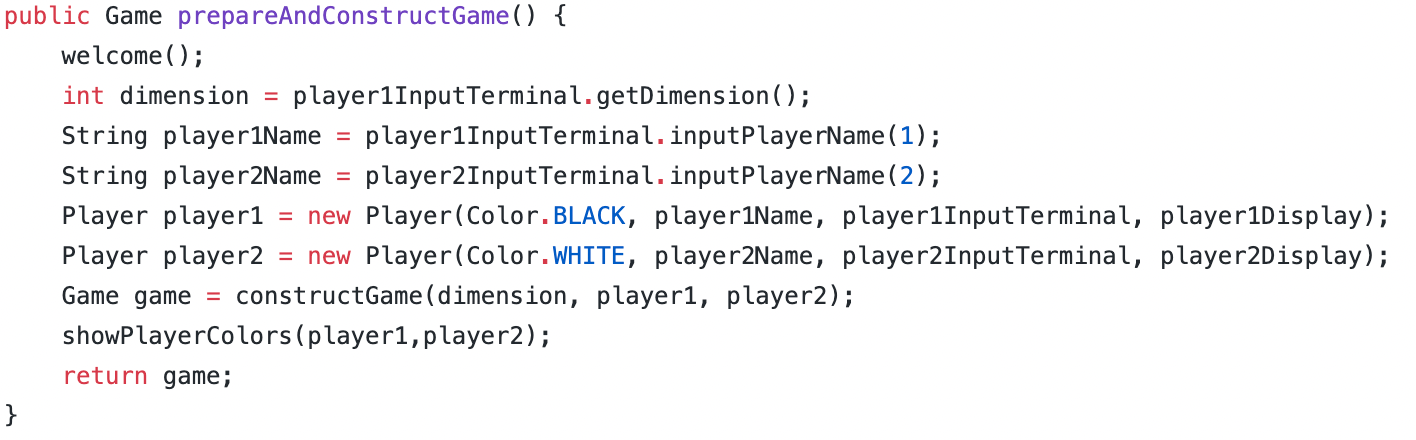
\includegraphics[scale=0.4]{images/prepareandconstruct.png}
\begin{columns}\hspace{-0.5cm}
			\column{0.4\textwidth}
			\begin{figure}
				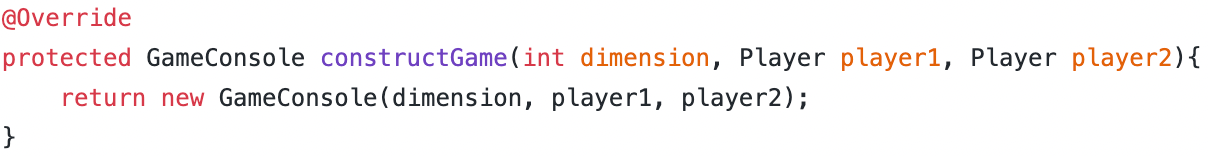
\includegraphics[scale=0.24]{images/constructconsole.png}
				\caption*{\hspace{-0.2cm}\texttt{GameInitializerConsole}}
			\end{figure}
					
			\column{0.5\textwidth}
			\begin{figure}
				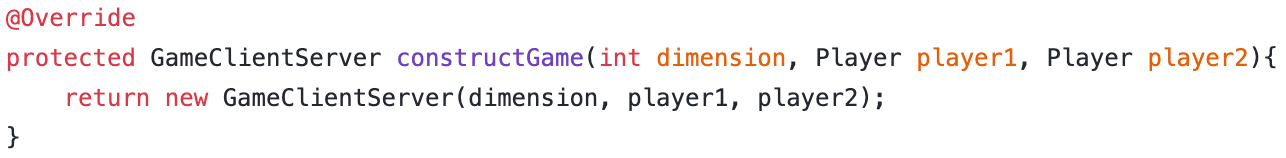
\includegraphics[scale=0.24]{images/constructcs.png}
				\caption*{\texttt{GameInitializerClientServer}}
			\end{figure}
		
	\end{columns}

\end{frame}

\begin{frame}{Comparing \texttt{GameConsole} and \texttt{GameClientServer}}
Client-Server version has to differentiate the messages for the two players:
\begin{columns}
			\column{0.5\textwidth}
			\begin{figure}
				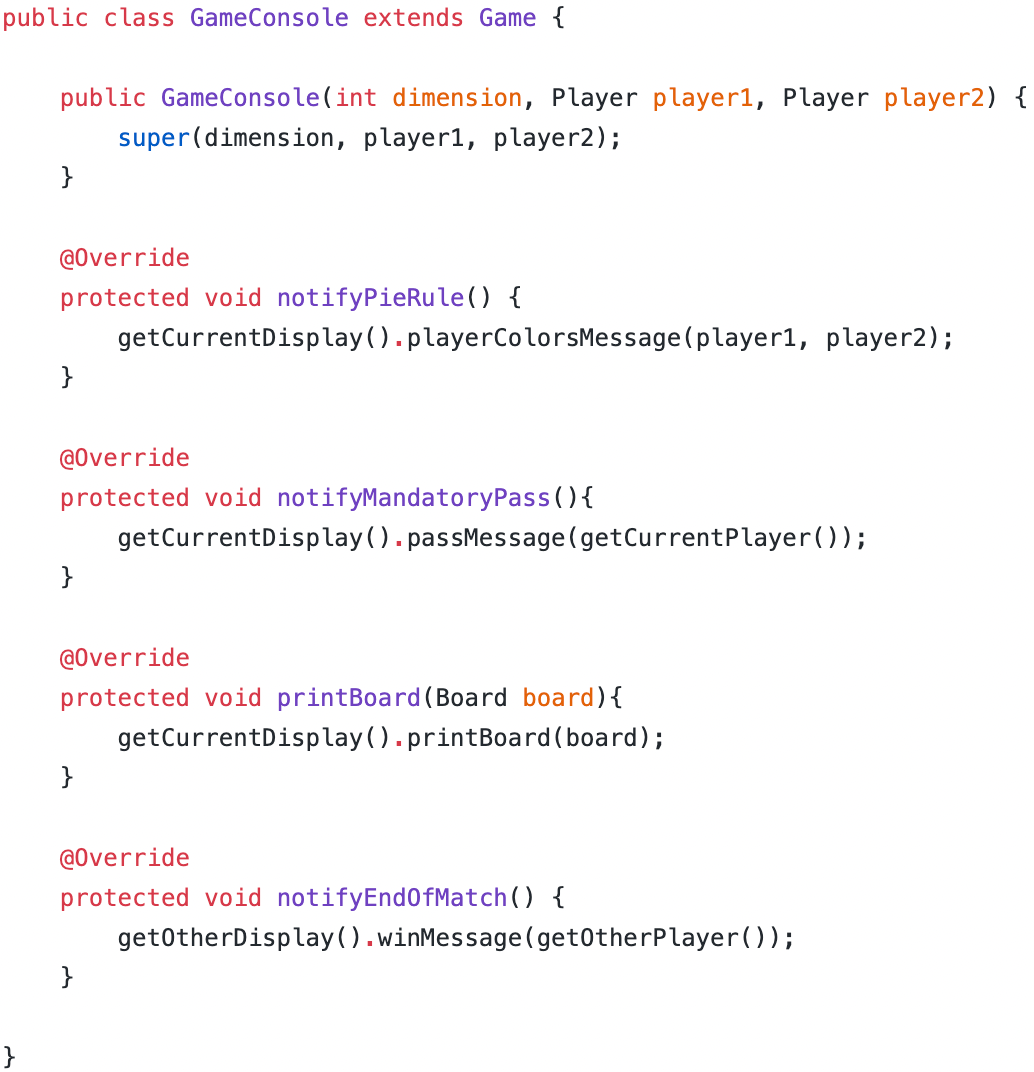
\includegraphics[height=5cm, keepaspectratio]{images/gameconsole.png}
				\caption*{\texttt{GameConsole}}
			\end{figure}
					
			\column{0.5\textwidth}
			\begin{figure}
				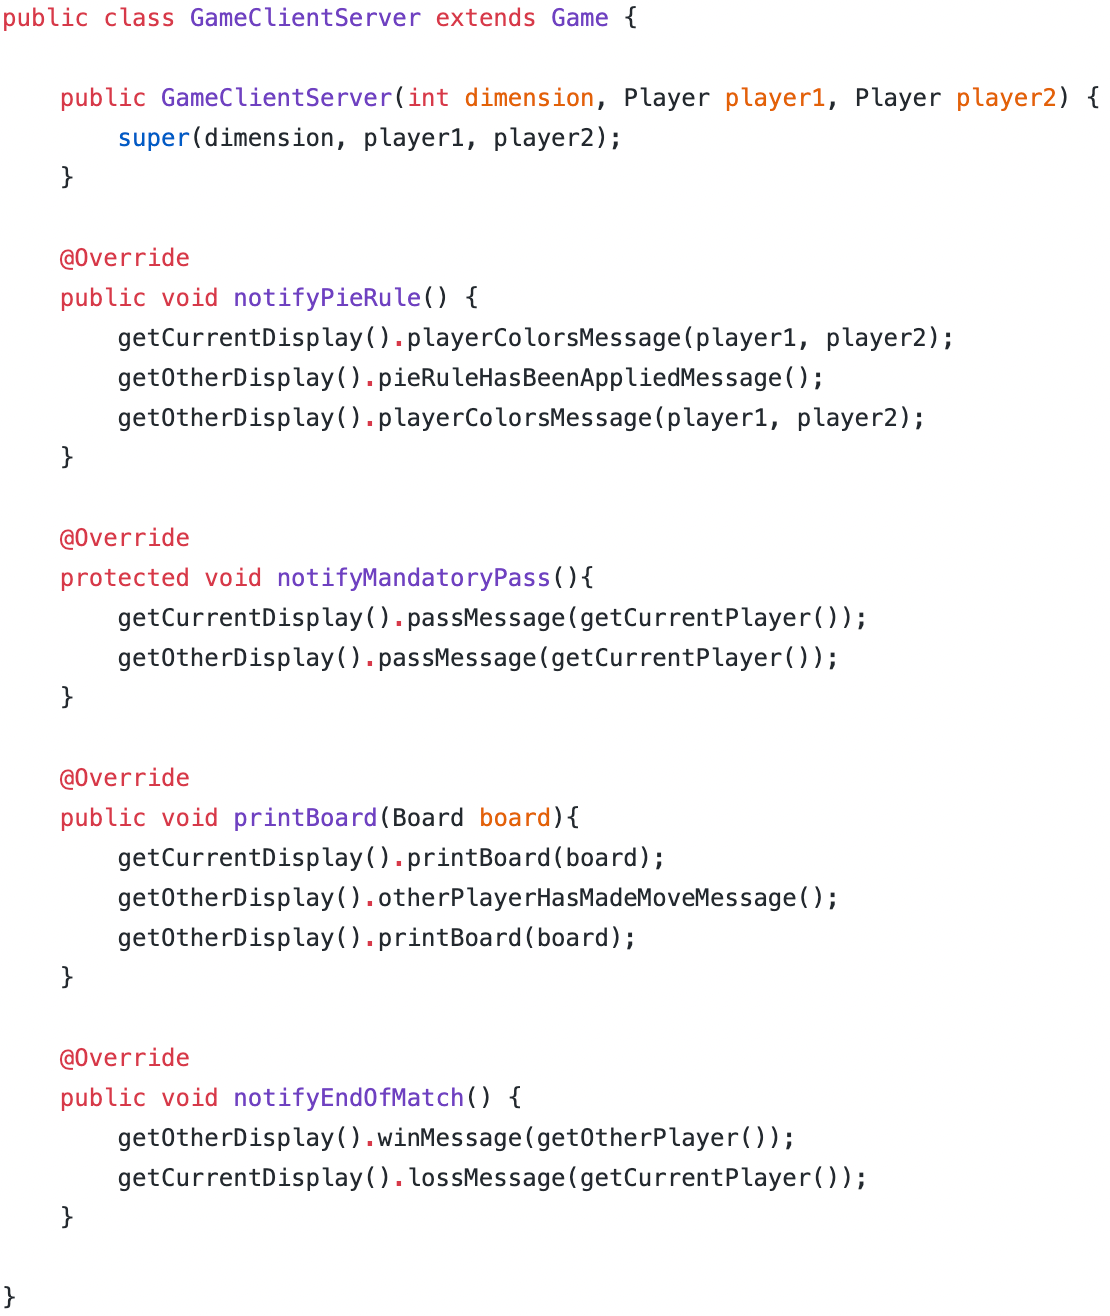
\includegraphics[height=5cm, keepaspectratio]{images/gamecs.png}
				\caption*{\texttt{GameClientServer}}
			\end{figure}
		
	\end{columns}
\end{frame}

\begin{frame}{Testing the game}
FOTO DEL TEST?
\end{frame}









     
\end{document}